\chapter{Vergleich von 4G EPS-AKA und 5G-AKA}
\label{chap:3}

Das 4G EPS-AKA Protokoll ist Teil des 4G Standards, dem Vorgänger des 5G Standards, zu dem das 5G-AKA Protokoll gehört.
Beide Protokolle sind \textit{Authentication and Key Agreement} Protokolle und haben somit einiges an Gemeinsamkeiten, sie unterscheiden sich aber auch voneinander.

\section{Beschreibung des 4G EPS-AKA Protokolls}

Das 4G EPS-AKA Protokoll ist eines von mehreren Protokollen des 4G Standards.
Es ist für den Austausch eines Schlüssels zur weiteren Kommunikation zuständig.

Die Entitäten des 4G EPS-AKA Protokolls lassen sich in die drei Teile \textit{User Equipment}, \textit{''Serving Network''} und \textit{''Home Network''} unterteilen.
Das \gls{ue} ist das \textit{User Equipment} und stellt die Komponenten dar, die sich bei dem Benutzer befinden, z.B. im Smartphone.
Die \gls{enodeb} und dei \gls{mme} sind Teil des \textit{''Serving Network''} und befinden sich bei dem Netzbetreiber, der das Netzwerk dem Benutzer zur Verfügung stellt.
Der \gls{hss} ist Teil des \textit{''Home Network''} und befindet sich bei dem Netzbetreiber, der dem Benutzer z.B. die SIM-Karte ausgestellt hat. %A Comparative Introduction of 4G and 5G Authentication

\subsection{Das Protokoll}

\begin{figure}[H]
  \centering
  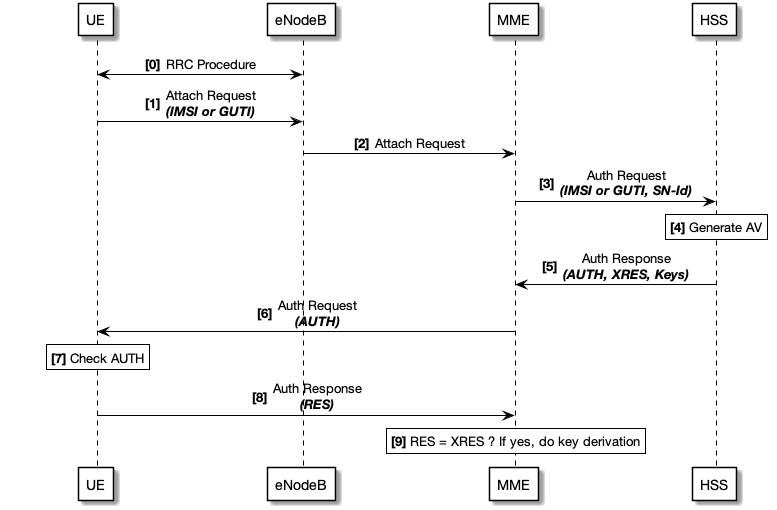
\includegraphics[width=\textwidth]{uml/4g-protocol_v1.png}
  \caption{Erfolgreiche Authentifikation}
  \label{fig:protocol_v1}
\end{figure}

\section{Unterschiede von 4G EPG-AKA und 5G-AKA}
